\documentclass{article}

\usepackage{palatino}
\usepackage{amsmath}
\usepackage{amsthm}
\usepackage{amssymb}
\usepackage{mathtools} 
\usepackage{mathrsfs}
\usepackage{enumitem}
\usepackage{mathtools}
\usepackage{fancyhdr}
\usepackage{mathpartir}
\usepackage{framed}

\newtheorem{theorem}{Theorem}


% https://tex.stackexchange.com/questions/235525/how-to-write-these-symbols-double-vee-wedge-and-bracket
\DeclareMathOperator*{\bigdoublewedge}{\bigwedge\mkern-15mu\bigwedge}

\newcommand{\scM}{\mathscr{M}}
\newcommand{\scP}{\mathscr{P}}
\newcommand{\mcI}{\mathcal{I}}
\newcommand{\mcO}{\mathcal{O}}
\newcommand{\ff}{\mathbb{F}}
\newcommand{\mm}{\mathbb{M}}
\newcommand{\nn}{\mathbb{N}}

\title{A Theory of Programs \\ 

\large{
    An Outline of Joint Work by
}}
\author{J.W. De Bakker and Dana Scott}
\date{IBM Seminar, Vienna, August 1969}

\begin{document}

\begin{center}
    \large{\textit{A note from the typesetter}} \\
    \hrule
\end{center}

Care has been taken to preserve the original intent as much as possible but this document is not intended to be historical- rather only a more convenient setting to read  Scott and de Bakker's unpublished work at IBM Vienna 1969. The original scan can be found at: 

\begin{framed}
https://www.cs.ox.ac.uk/strachey100/Strachey\_booklet.pdf \\

Klop, J.W, Meijer, J.J.C, \& Rutten, J.J.M.M (Eds.). (1989). J.W. de Bakker, 25 jaar semantiek : liber amicorum. (J.W Klop, J.J.C Meijer, \& J.J.M.M Rutten, Eds.). CWI.
\end{framed}


\maketitle

\section{Machines}

A \underline{machine} is a structure 
\begin{equation*}
    \scM = (\mcI, \mcO, F_0, p_0, F_1, p_1, \ldots)
\end{equation*}

of \textit{partial} functions for which there exist (uniquely determined) sets $X$, $M$, $Y$, such that 
\begin{align*}
    \mcI & : X \to M && \hspace{-100pt} \textrm{\textit{(the input function)}} \\
    \mcO & : M \to Y && \hspace{-100pt}\textrm{\textit{(the output function)}} \\
    F_i & : M \to M && \hspace{-100pt}\textrm{\textit{(the operations)}} \\
    p_j & : M \to \{0, 1\} && \hspace{-80pt}\textrm{\textit{(the tests)}}. \\
\end{align*}

As a diagram, we can write
\begin{center}
    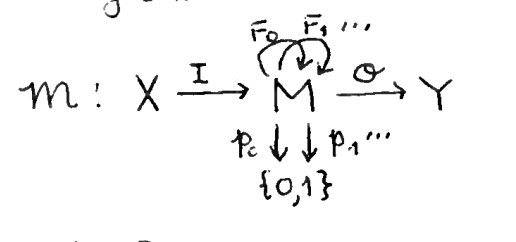
\includegraphics[width=230pt]{dg1.png}
\end{center}

\section{Computations}

A \underline{computation} (from $x \in X$ to $y \in Y$) is a finite sequence 
\begin{equation*}
    \xi_0, F_{i_0}, \xi_1, F_{i_1}, \xi_2, \ldots, \xi_{k-1}, F_{i_{k-1}}, \xi_k
\end{equation*}
whete each $\xi_\ell \in M$ and $\xi_{\ell+1} = F_{i_l}(\xi_\ell)$ for $\ell < k$ (and where $I(x) = \xi_0$ and $O(\xi_k) = y$).

\section{Programs}

Informally, a \underline{program} is a ``method'' of selecting \textit{at most} one computation starting from each $x \in X$. Thus, a program $\scP$ associates to the machine $\scM$ a partial function 
\begin{equation*}
    \scP(\scM) : X \to Y.
\end{equation*}

Programs must be defined ``independently'' of particular machines, and indeed we can identify the program with this mapping from machines to functions. A program as a mapping must satisfy some general conditions to be mentioned later. First we give some examples. 

\section{Flow Diagrams}

It is intuitively clear that, given an arbitrary machine $\scM$, this diagram allows us to generate for each $x \in X$ at most one computation, offered by following the ``flow'' of the diagram. We say that the diagram (a ``syntactical'' object) \underline{defines} a program (a mathematical object). 

\begin{center}
    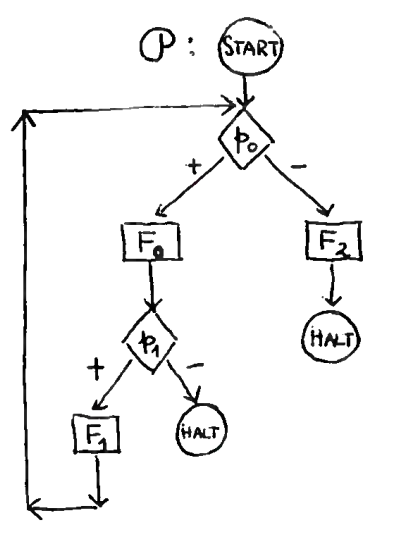
\includegraphics[width=100pt]{dg2.png}
\end{center}

\section{Procedures}

\begin{equation*}
    \scP : \begin{cases}
        P_0 \Rightarrow (p_0 \to F_0; P_1, F_2)\\
        P_1 \Rightarrow (p_1 \to F_1; P_0, E)\\
    \end{cases}
\end{equation*}

Here we have a system of procedure declarations (where by convention $P_0$ is the ``principal'' one). $(p \to P, P')$ is the \underline{conditional expression}; $P;P'$ is \underline{composition} ($P$ followed by $P'$); and $E$ is the symbol for the \underline{identity function}. The above system defines the same program as the flow diagram [\textit{in section 4}]. 

\section{While Statements}
\begin{equation*}
    \scP': (p_0 * (p_1 * F_1); F_0); (p_2 * F_2)
\end{equation*}
Read ``$(p * P)$'' as ``\underline{while} $p$ \underline{do} $P$''. The same program can be defined by flow diagrams or by procedures

\begin{center}
    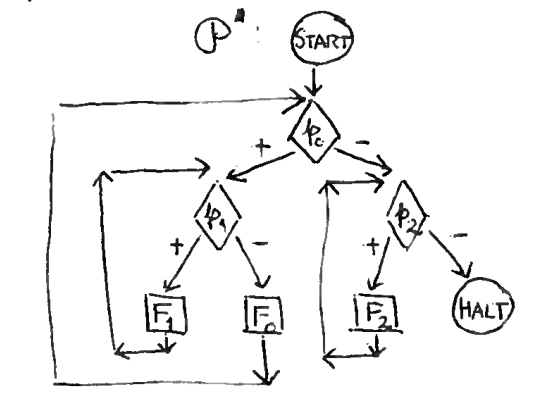
\includegraphics[width=200pt]{dg3.png}
\end{center}
\begin{equation*}
    \scP' : \begin{cases}
        P_0 \Rightarrow (p_0 \to P_1; P_0, P_2) \\
        P_1 \Rightarrow (p_1 \to F_1; P_1, F_0) \\
        P_2 \Rightarrow (p_2 \to F_2; P_2, E) \\
    \end{cases}
\end{equation*}

\section{Equivalences}
Two programs $\scP$ and $\scP'$ are \underline{equivalent} \textit{on} a machine $\scM$ iff $\scP(\scM) = \scP'(\scM)$. They are (\underline{strongly}) \underline{equivalent} iff they are equivalent on \textit{all} machines; that is iff $\scP = \scP'$. Two flow diagrams (systems of procedures, \underline{while} systements) are equivalent iff they define equivalent programs.

\begin{theorem}
    Every program defined by a \underline{while} statement is (effectively) equivalent to one defined by a flow diagram, \textit{but} there is a flow diagram that defines a program \underline{\underline{not}} defined by any \underline{while} statement. 
\end{theorem}

\begin{theorem}
    (the same for flow diagrams and procedures)
\end{theorem}

\begin{theorem}
    It is (effectively) decidable whether two flow diagrams are equivalent
\end{theorem}

\begin{theorem}
    It is (effectively) decidable whether a system of procedures defines the null program $\Omega$.
\end{theorem}

\noindent\textbf{Problems:} Is it (effectively) decidable whether two procedures are equivalent? Is it decidable whether a procedure is equivalent to some flow diagram? A flow diagram to a \underline{while} statement?

\section{General Properties}

We write $\scM \subseteq \scM'$ iff $\scM$ and $\scM'$ have the same sets $X$, $M$, $Y$ and have operations and tests $F_i \subseteq F_i'$ and $p_i \subseteq p_i'$ for all $i, j$ (that is, $F'_i$ is consistent with, but more defined than $F_i$). 

\begin{enumerate}[label=(\Roman*). ]
    \item $\scM \subseteq \scM'$ implies $\scP(\scM) \subseteq \scP(\scM')$ \\
            (Property (I) can be generalized by defining \underline{morphisms} $\varphi : \scM \to \scM'$ between machines. See below.) \\
        \item If for $\scM_n \subseteq \scM_{n+1}$ for $n = 0, 1, 2, \ldots$ then 
            \begin{equation*}
                \scP \left( \bigcup\limits_{n=0}^\infty \scM_n \right) = \bigcup\limits_{n=0}^\infty \scP(\scM_n)
            \end{equation*}
            (Property (II) can be generalized to directed unions (and, no doubt, to direct limits)). \\
    \end{enumerate}
     Write $\scM^{(n,m)}$ for the result of modifying $\scM$ by replacing $F_i$ and $p_j$ by the \underline{totally undefined} functions for $i \geq n$ and $j \geq m$. \\
    \begin{enumerate}[resume, label=(\Roman*). ]
        \item For every program $\scP$ there exists $n$, $m$ such that for all machines $\scM$
            \begin{equation*}
                \scP(\scM) = \scP(\scM^{(n,m)})
            \end{equation*}
\end{enumerate}

The above are defined for procedures, and (suitably generalized) ought to be taken as ``axiomatic'' for the notion of program. 

\section{Categories} 

Let $\ff$ be the caregory whose \underline{objects} are \textit{partial functions} $F: X \to Y$ and whose \underline{morphisms} $\varphi: F \to F'$ are pairs $\varphi = (\varphi^\downarrow, \varphi^\uparrow)$ where 
\begin{gather*}
    \varphi^\downarrow : X \to X' \\ 
    \varphi^\uparrow : Y' \to Y \\ 
    F \subseteq \varphi^\downarrow; F'; \varphi^\uparrow
\end{gather*}

\begin{center}
    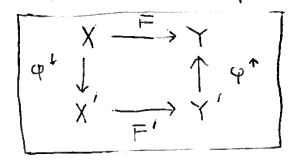
\includegraphics[width=120pt]{dg4.png}
\end{center}


(Here, ``$;$'' denotes \underline{composition of relations} so that $(F;G)(x) = G(F(x))$ in the case of functions). \\

Let $\mm$ be the category whoste \underline{objects} are \textit{machines} and whose \underline{morphisms} $\varphi: \scM \to \scM'$ are triples $\varphi = (\varphi^\downarrow, \varphi^\square, \varphi^\uparrow)$ where $\varphi^\downarrow : X \to X'$ and $\varphi^\square: M \to M'$ and $\varphi^\uparrow : Y' \to Y$ and where for all $i, j$:
\begin{gather*}
    \mcI \subseteq \varphi^\downarrow; \mcI'; (\varphi^\square)^{-1} \\
    \mcO \subseteq \varphi^\square; \mcO'; (\varphi^\uparrow)^{-1} \\
    F_i \subseteq \varphi^\square; F_i'; (\varphi^\square)^{-1} \\ 
    p_j \subseteq \varphi^\square; p_j' \\
\end{gather*}
(Here, ``$\mbox{}^{-1}$'' denotes \underline{converse} of a relation) \\ 

\begin{center}
    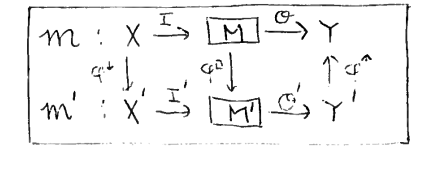
\includegraphics[width=220pt]{dg5.png}
\end{center}

Let $\scP$ be a program and let $\varphi : \scM \to \scM'$. Define $\scP(\varphi) = (\varphi^\downarrow, \varphi^\uparrow)$ where $\varphi = (\varphi^\uparrow, \varphi^\square, \varphi^\downarrow)$. 
\begin{theorem}
    If $\varphi : \scM \to \scM'$ in the category $\mm$, then $\scP(\varphi): \scP(\scM) \to \scP(\scM')$ in the category $\ff$.
\end{theorem}

This is at least clear for programs defined by procedures; it should be taken as ``axiomatic'' in general. Thus it follows that $\scP: \mm \to \ff$ is a \textit{functor} between categories. This is the proper generalization of property (I) above as a function $\scP$ ought to be rather ``continuous'' in some suitable sense. \\ 

If $\scM : X \xrightarrow{\mcI} \fbox{$M$} \xrightarrow{\mcO} Y$, define $[\scM] : M \xrightarrow{E} \fbox{$M$} \xrightarrow{E} M$ to be the machine with the same operations and tests but with $\mcI$, $\mcO$, $X$, $Y$ replaced with $E$, $E$, $M$, $M$ where $E$ is the identity on $M$. Then we have the result
\begin{equation*}
    (\mcI, E, \mcO) : \scM \to [\scM] \textrm{\quad in } \mm.
\end{equation*}

It was the ``obvious correctness'' of this relationship that motivated the above definitions. The categories $\mm$ and $\ff$ require much more study, however, before their usefulness can be determined. 

\section{Control Devices}

By \underline{control device} we shall understand a ``Boolean'' machine: 

\begin{center}
    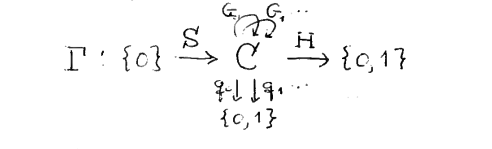
\includegraphics[width=220pt]{dg6.png}
\end{center}

\section{``Abstract'' programs}

Let $\nn = \{0, 1, 2, \ldots\}$ and let $\{0, 1\}^\infty$ be the set of all \underline{partially} defined infinite sequences of 0's and 1's. If $\scM$ is a machine and $\xi \in M$, define 

\begin{equation*}
  p(\xi) = (p_0(\xi), p_1(\xi), \ldots, p_n(\xi), \ldots) \in \{0,1\}^\infty  
\end{equation*}

An ``abstract'' program $\scP_{f,g}^\Gamma$ is defined by giving a control device $\Gamma$ (generally \underline{fixed} so that a definite class of programs is considered) and two functions 

\begin{equation*}
    f,g : \{0,1\}^\infty \times \{0, 1\}^\infty \to \nn
\end{equation*}

such that the selected computations of $\scP_{f,g}^\Gamma$ on a machine $\scM$ (in the notation of page 1) are those for which there exist (uniquely determined) computations

\begin{equation*}
    \gamma_0, G_{j_0}, \gamma_1, G_{j_1}, \ldots, \gamma_{k-1}, G_{j_{k-1}}, \gamma_k
\end{equation*}

on the machine $\Gamma$ where for $\ell \leq k$

\begin{gather*}
    i_\ell = f(p(\xi_\ell), q(\gamma_ell)) \\ 
    j_\ell = g(p(\xi_\ell), q(\gamma_ell)) \\ 
    \gamma_0 = \mathcal{S}(0), \mathcal{H}(\gamma_\ell) = 0, \text{\quad for } \ell < k \\
    \mathcal{H}(\gamma_k) = 1
\end{gather*}
Thus $\mathcal{S}$ and $\mathcal{H}$ control the \underline{start} and \underline{halt} and $f$ and $g$ tell where to look for the next operation to execute. We need $\Gamma$ as a ``memory'' to keep track of where we are in the intermediate stages of ``reading'' the text of the program definition. Assuming that $f$ and $g$ are ``finitely given'' (i.e. depend on a fixed bounded number of coordinates of $p(\xi)$ and $q(\xi)$), we can then prove that $\scP_{f,g}^\Gamma$ is a functor with basic properties (I), (II), (III), (we need some slight \underline{consistency} conditions on $f$ and $g$). \\

\noindent\textbf{Conjecture:} There are a few more ``nice'' properties (like (I), (II), (III)) such that any functor $\scP: \mm \to \ff$ having these properties is of the form $\scP_{f,g}^\Gamma$. \\

Note: in this abstract setting is is convenient to make the harmless convention that on all machines $\scM$ we have $F_0 = E$, the identity on $M$. 

\section{Examples}

The ``abstract'' version of the \underline{flow diagram} uses the control device where

\begin{align*}
    \mathcal{C} &= \{-1, 0, 1, 2, \ldots\} \\
    \mathcal{S}(0) &= 0 \\
    \mathcal{G}_j(\gamma) &= j - 1 \\ 
    q_j(\gamma) & = \begin{cases}
        1 & \gamma = j \\
        0 & \textrm{otherwise}
    \end{cases} \\
    H(\gamma) & = \begin{cases}
        1 & \gamma = -1 \\
        0 & \textrm{otherwise}
    \end{cases} \\
\end{align*}

The ``abstract'' version of the \underline{procedure} uses the more general control device where

\begin{align*}
    \mathcal{C} &= \{0, 1, 2, \ldots \}^{*} = \{\sigma_0, \sigma_1, \sigma_2, \ldots \} \\
    \mathcal{S}(0) &= 0 \\
    \mathcal{G}_j(n\gamma) &= \sigma_j \gamma \\ 
    q_j(n\gamma) & = \begin{cases}
        1 & n = j \\
        0 & \textrm{otherwise}
    \end{cases} \\
    H(\gamma) & = \begin{cases}
        1 & \gamma = \Lambda \\
        0 & \textrm{otherwise}
    \end{cases} \\
\end{align*}

where $\Lambda$ is the \underline{null} sequence and the $\sigma_n$ represent some (recursive!) enumeration of the finite sequences of integers. (In other words, the control of a procedure computation is in general a \underline{push-down} store). 

\section{Deductions}

For the time being we restrict attention to \underline{procedures} and ask how it can be established where two of them are \textit{equivalent}. In one sense the question is answered because we have given a completely precise definition of the program defined by a procedure with the aid of a certin control device. That answer is not too helpful, because no simple ``methods'' of proof for proving equivalence are provided by the bare definition. Two different (though related) deductive systems are presented below which might be called the ``algebraic'' and the ``second-order relational'' theories. The algebraic method is more efficient for proving \underline{equivalences}; while the relational method is better for problems of \underline{correctness}. It is not known whether an algebraic theory can be complete- because if it is, and if it's theorems are recursively enumerable, then we would have a recursive decision method for equivalence. The relational theory \underline{is} complete- because we use second-order logic, but the theorems are \textit{not} enumerable.  

\section{The Algebraic Theory}
\subsection{Language}
Lower-case letters are \underline{Boolean variables} (mostly we use $p$, $q$, $r$). Upper-case letters are \underline{predicate variables}, except we use $E$ and $\Gamma$ as \underline{constants}. Compound \underline{terms} are constructed from upper-case letters by these three operations
\begin{align*}
    (p \to \tau, \sigma) \hspace{20pt} \tau; \sigma \hspace{20pt} \mu X [\tau] 
\end{align*}
where in place of $p$ we can have any Boolean and in place of $X$ any procedure variable. The first is the \underline{conditional expression}, the second, a \underline{composition}; and the third a \underline{variable binding operator} $\mu$ whose meaning is explained below. Atomic formulas are either \underline{equations} $\tau = \sigma$ or \underline{inclusions} $\tau \subseteq \sigma$. Lists $\Phi_0, \Phi_1, \ldots, \Phi_{n-1}$ of atomic forumulas are used as short-hand for the conjugation $[\Phi_0, \Phi_1, \ldots, \Phi_{n-1}]$. \underline{Theorems} are of the form of implications $\Phi \vdash \Psi$ between lists. We use for simplicity in these notes the usual notation $\tau(X, Y)$, $\Phi(X, Z)$, $\Psi(X, \tau(X))$ to indicate (roughly!) free variables and results of substitutions. 

\subsection{Validity}
Consider an implication $\Phi \vdash \Psi$. Suppose the \underline{free} variables are $p_0, p_1, p_2, \ldots$ and $F_0, F_1, F_2, \ldots$. The implication is \underline{valid} just in case for all sets $M$ and all systems $F_i : M \to M$ and $p_j : M \to \{0,1\}$ of partial functions and predicates on $M$, \underline{if} $\Phi$ is \textit{true} for these \underline{then} so is $\Psi$. Now a list is true iff all it's terms are. An atomic $\tau = \sigma$ is true iff $\tau$ and $\sigma$ denote the \underline{same} function on $M$ into $M$. An atomic $\tau \subseteq \sigma$ is true iff $\tau$ denotes a function \underline{included} in that denoted by $\sigma$. Thus, given the value of the free variables we need still only define what is the function \underline{denoted} by a term. $E$ denotes the \underline{identity} function. $\Omega$ denotes the \underline{empty} (``undefined'') function. \underline{Conditionals} and \underline{compositions} denote functions obtained from the denotations of the parts in the usual way. The special term $\mu X[\tau(X)]$ denotes the \underline{least} function $G$ such that $\tau(G) \subseteq G$ (``least'' in the sense of the partial ordering $\subseteq$). We shall see below why it always exists, and why it is of interest in connection with procedures. 

\begin{theorem}
    The set of valid implications is \underline{not} recursively enumerable (sorry!)
\end{theorem}

\noindent\textbf{Problem:} Is the set of $\vdash \Psi$ recursively enumerable (and \underline{hence} recursive)?

\subsection{Axioms and Rules} The axioms and rules for conjugations and rules are well known. As for $;$, $\subseteq$, $E$, $\Omega$ we give the axioms of a \underline{partially ordered semigroup with unit and zero}. 
\begin{align*} 
    & \vdash (p \to X, Y); Z = (p \to X; Z, Y; Z) \\
    & \vdash (p \to X, X) \subseteq X \\ 
    X \subseteq X', Y \subseteq Y' & \vdash (p \to X, Y) \subseteq (p \to X', Y') \\
    (p \to X, \Omega) \subseteq Z, (p \to \Omega, Y) \subseteq Z & \vdash (p \to X, Y) \subseteq Z
\end{align*} 
(\underline{Maybe} some others are required?? This point about conditionals is not too clean and needs more study.) For $\mu$ we have

\begin{mathpar}
    Y = \mu X [ \tau(X) ] \vdash \tau(Y) \subseteq Y \quad (\mu-\textrm{Axiom}) \\
    \infer{\Phi \vdash \Psi(\mu X[\tau(X)])}{\Phi \vdash \Psi(\Omega) \quad\quad \Phi, \Psi(X) \vdash \Psi(\tau(X))} \quad (\mu-\textrm{Rule}) 
\end{mathpar}
(in the rule $X$ is not free in $\Phi$). 

\subsection{Application}

Consider the following system of procedures 
\begin{equation*}
    \scP'' = \begin{cases}
        P_0 \Rightarrow \tau_0(P_0, P_1) \\ 
        P_1 \Rightarrow \tau_1(P_1, P_2) \\ 
        P_2 \Rightarrow \tau_2(P_2, P_0) \\ 
    \end{cases}
\end{equation*}
where the $\tau_i$ are terms with the $P_i$ and possibly other free variables. The $P_i$ variables, of course, play a special role, and the above ``rewrite'' rules mean that the $P_i$ should be computed as the ``least'' functions that result from replacing procedure ``call'' by the corresponding ``body''. Hence,
\begin{equation*}
    P_2 = \mu Z[\tau_2(Z, P_0)],
\end{equation*}
and then 
\begin{equation*}
    P_1 = \mu Y [\tau_1 (Y, \mu Z[\tau_2(Z, P_0)])],
\end{equation*}
and finally
\begin{equation*}
    P_0 = \mu X [\tau_0(X, \mu Y [\tau_1 (Y, \mu Z[\tau_2(Z, P_0)])])].
\end{equation*}
Thus the whole program can be defined by the algebraic expression on the right hand side. Proving equations between expressions, then, \underline{is} proving equivalence of programs. 

\subsection{Justification}
With a combination of results proved within the system and semantics \underline{outside} the theory, we will see that the axioms are valid and that the rules preserve validity. Later we give some examples of particular equivalence proofs. 

\begin{enumerate}
    \item $X \subseteq X' \vdash \tau(X) \subset \tau(X')$ \\ 
        \textit{Proof:} The theorem must first be generalized to any number of variables and then proved by induction on the complexity of the term $\tau$. The cases of conditionals and composition are already assumed as (obviously valid) axioms. For the $\mu$-operator we do a representative special case. Thus assume $\sigma(X,Y)$ monotone in both variables, and consider $\tau(X)$ to be $\mu X[\sigma(X, Y)]$. By the first $\mu$-axiom 
        \begin{equation*}
            \vdash \sigma(X', \tau(X')) \subseteq \tau(X')
        \end{equation*}
hence by assumption of $\sigma$
        \begin{equation*}
            X \subseteq X' \vdash \sigma(X', \tau(X')) \subseteq \tau(X') \subseteq \tau(X').
        \end{equation*}
  We can again apply the monotonicity of the term $\sigma$ to derive:
        \begin{equation*}
            X \subseteq X', Y \subseteq \tau(X')  \vdash \sigma(X, Y) \subseteq \tau(X').
        \end{equation*}

        Note that $X \subseteq X' \vdash \Omega \subseteq \tau(X')$ is trivial; thus by the rule for the $\mu$-operator we have 
        \begin{equation*}
            X \subseteq X' \vdash \mu Y [\sigma(X,Y)] \subseteq \tau(X'),
        \end{equation*}
        which is the desired result for $\tau$. \\


        \underline{Discussion.} We proved monotonicity by the axioms and rules for $\mu$, but this proof also helps (in part) to establish the validity of these principles. In our calculus the expressions repsresent \underline{monotonic operations} on partial functions. It is well-known that such operations have \underline{minimal fixed points}. Speaking informally:
        \begin{align*}
            \mu X[\tau(X)] 
            & = \bigcap \; \{X :  \tau(X) \subseteq X \} \\
            & = \bigcup\limits_{n=0}^\infty \tau^n(\Omega)
        \end{align*}
        where $\tau^n(\Omega) = \overbrace{\tau(\tau(\ldots \tau(}^{n \textrm{ times}} \Omega) \ldots ))$. The second equation, which justifies the special case of the rule used in the proof of (1), is correct because the operation is also \underline{continuous} in this sense (speaking outside the theory)
        \begin{equation*}
            \tau\left( \bigcup\limits_{n=0}^\infty X_n \right) = \bigcup\limits_{n=0}^\infty \tau(X_n)
        \end{equation*}
        whenever $X_0 \subseteq X_1 \subseteq \cdots \subseteq X_n \subseteq \cdots$. This is clear for conditionals and compositions, but again must be established for $\mu$'s. Once conitnuity is understood, the validity of the full rule for $\mu$ (which we may call the \underline{induction rule}) follows easily. \\

    \item Fixed Point Properties
        \begin{align*}
            Y = \mu X [\tau(X) ] & \vdash \tau(Y) = Y \quad \textrm{ and} \\
            \tau(Y) \subseteq Y & \vdash \mu X [ \tau(X) ] \subseteq Y
        \end{align*}
        The proof uses monotonicity and induction as in the proof of (1).  \\

    \item Systems of Fixed Points
        \begin{align*}
            & X = \mu X [ \tau(X, \mu Y[\sigma(X,Y)])], \\
            & Y = \mu Y [ \sigma(X, Y)], \\
            & \tau(X', Y') \subseteq X', \sigma(X', Y') \subseteq Y' \vdash \\
            & \tau(X, Y) \subseteq X \subseteq X', \sigma(X,Y) \subseteq Y \subseteq Y' \\
        \end{align*}
        \textit{Proof:} ``Assume'' the hypothesis. Then $\tau(X, \mu Y[\sigma(X,Y)]) \subseteq X$ and so $\tau(X,Y) \subseteq X$. Also $\sigma(X,Y) \subseteq Y$. Let $Y'' = \mu Y[\sigma(X', Y)]$. Then $Y'' \subseteq Y'$ and so $\tau(X', Y'') \subseteq X'$. But then $X \subseteq X'$ and so $\sigma(X, Y') \subseteq Y'$. Finally $Y \subseteq Y'$. \\

        \underline{Discussion.} The above theorems on minimal fixed points can be extended to systems with \underline{any number} of procedure declarations. 
\end{enumerate}

\subsection{Examples:}
We define \underline{while} as $(p * F) = \mu X [(p \to F; X, E)]$
\begin{enumerate}[label=(\alph*)]
    \item $(p*F);G = \mu Y [(p \to F; Y, G)]$.
        \textit{Proof:} By definition $(p * F) = (p \to F; (p*F), E)$. Hence $(p * F); G = (p \to F; (p*F); G, G)$. Therefore, $\mu Y [(p \to F; Y, G)] \subseteq (p*F); G$. To prove the opposite inclusion, first let $Y = \mu Y [( p \to F; Y, G)]$. By induction it is enough to show $\Omega; G \subseteq Y$ (obvious!) and $X; G \subseteq Y \vdash (p \to F; X, E); G \subseteq Y$. So assume $X; G \subseteq Y$. But $(p \to F; Y, G) \subseteq Y$. Thus $(p \to F; X, E); G =  (p \to F; X; G, G) \subseteq Y$. \\
    \item $p*(p*F) = p * (F; p*F)$
        \textit{Proof:} Let $L$ be the left-hand side and $R$ be the right. Then
        \begin{align*}
            L &= (p \to (p * F); L, E) \\
            &= (p \to (p \to F; (p * F), E); L, E) \\
            &= (p \to F; (p*F); L, E) \\
        \end{align*}
        thus $R \subseteq L$. Next
        \begin{align*}
            R &= (p \to F; (p*F); R, E) \\
            &= (p \to (p \to F; (p*F), E); R, E) \\
            &= (p \to (p*F); R, E)
        \end{align*}
        thus $L \subseteq R$ and $L=R$ follows. \\
        
    \item $(p*F);(p \to G, H) = (p*F); H$ \\
    \item $(p*F);(p*G) = p*F$ \\
    \item $p*(p*F) = p*F$ \\
\end{enumerate}
all of these follow from (i) and the method shown for (ii). 

\section{The Relational Theory}

Functions are, after all, \underline{relations}. Thus it must be possible to axiomatize the functions defined by program expressions, hopefully without the minute detail of the definitions containing control devices which are closer to the ideas of the implementation. We do this for procedures.

\subsection{Language}

We use a standard second-order predicate calculus with equality and notaional conventions corresponding to our language of procedure declarations. In particular we employ the following style of variables and non-logical constants:

\begin{itemize}
    \item \underline{Individual} variables $\xi, \eta, \zeta, \xi', \eta', \ldots$
    \item 1-\underline{place} predicate constants $p, \bar{p}, q, \bar{q}, \pi, \bar{\pi}, \ldots$
    \item \underline{Binary relation} variables $R$, $S$, $T$, $X$, $Y$, $Z$
    \item \underline{Binary relation} constants $E$, $\Omega$, $P_0$, $P_1$, $P_2$, $\ldots$
    \item \underline{Relational} operations $(R;S)$, $(p \to R, S)$
    \item \underline{Atomic Formulas}: \underline{equations} plus 
        \begin{equation*}
            R \subseteq S \quad\quad p(\xi) \quad\quad \xi R \eta
        \end{equation*}
        (where in place of $R$ and $S$ we can have relational terms and in place of $p$ the other $\bar{p}, q, \bar{q}, \ldots$ and in place of $\xi$, $\eta$ any individual variables.) 
\end{itemize}

\subsection{Validity and Deduction}

This is the usual notion from second-order logic; we do, however, have a few non-logical axioms to suit the application to procedures. Remember that the valid formulas are \underline{not} recursively enumerable in second-order logic. \\

\subsection{General Axioms}
We assume the following definitions and axioms

\begin{enumerate}[label=(\arabic*)]
    \item $\neg \exists \xi \; [p(\xi) \wedge \bar{p}(\xi)]$ (sim for $q, \pi, \ldots$)
    \item $\forall \xi, \eta \; [\xi E \eta \leftrightarrow \xi = \eta]$
    \item $\neg \exists \xi, \eta \; [\xi \Omega \eta]$
    \item $\forall \xi, \eta \; [ \xi (R; S) \eta \leftrightarrow \exists \zeta \; [\xi R \zeta \wedge \zeta S \eta]]$
    \item $\forall \xi, \eta \; [ \xi (p \to R, S) \eta \leftrightarrow [ [p(\xi) \wedge \xi R \eta] \vee [\bar{p}(\xi) \wedge \xi S \eta] ]]$
    \item $R \subseteq S \leftrightarrow \forall \xi, \eta \;[\xi R \eta \to \xi S \eta]$
\end{enumerate}
(where $R$, $S$ should be universally quantified). \\

The meaning of the axioms is clear except maybe for (1). Here the pair $p, \bar{p}$ is to represent a partial predicate (by convention all predicates in logic are total). The $p$ is the \underline{true} part and the $\bar{p}$ is the \underline{false} part. They must be disjoint -- but that is the only requirement. We do not need any similar tricks for partial functions since they are just relations in a straight-forward way. 

\subsection{Special Axioms}
Consider a program $\scP$ defined by a system of declarations
\begin{equation*}
    \scP = \begin{cases}
        P_0 \Rightarrow \tau_0(P_0, \ldots, P_n) \\
        \quad \vdots \\
        P_n \Rightarrow \tau_n(P_0, \ldots, P_n) \\
    \end{cases}
\end{equation*}

Corresponding to this system we have

\begin{align*}
    (i_\scP) \quad\quad & [\tau_0(P_0, \ldots, P_n) \subseteq P_0  \wedge \tau_1(P_0, \ldots, P_n) \subseteq P_1  \wedge \ldots \wedge \tau_n(P_0, \ldots, P_n) \subseteq P_n] \\
    (ii_\scP) \quad\quad &\forall R \; \left[ \bigdoublewedge\limits_{i=0}^n \; [\tau_i (R_0, \ldots, R_n) \subseteq R_i ] \to \bigdoublewedge\limits_{i=0}^n [P_i \subseteq R_i]] \right]
\end{align*}

\subsection{Justification}
Given a system of procedures, we have mereley assumed -- in second-order langauge -- that $P_i$ are the \underline{least} relations where $\tau_i(P_0, \ldots, P_n) \subseteq P_i, i=0,1,\ldots,n$. This was the same idea as the algebraic theory -- except we do not have the $\mu$-operator. We could introduce it, and then all the algebraic principles could be proved from the second-order axioms. 

% Oblset
\textbf{Remark:} Given that the \underline{free} variables of the procedures are $F_0, F_1, F_2, \ldots$ (our usual convention) we might want to assume that they are \underline{partial functions} (our usual convention). We should have them, as general axioms,

\begin{equation*}
    \forall \xi, \eta, \eta'\;[\xi F_i \eta \wedge \xi F_i \eta' \rightarrow \eta = \eta']
\end{equation*}

These axioms do not seem to make too much difference, however. 

\subsection{Applications}
Suppose $\scP$ and $\scP'$ are programs defined by procedures (where, say, in the second system we use constants $P_0', P_1', \ldots$). The equivalence problem is to deduce, therefore, the statement $P_0 = P_0'$ from \underline{all} the axioms combined. The use of second-order deductions does not seem, however, any more convenient than the algebraic method for such equivalence. The point of the second-order system lies, rather, in the fact that more and different kind of problems can be expressed within it. \\

\subsection{While Statements}
 For the sake of illustration we restruct our attention to \underline{while} statements. These are special procedures, and we can introduce them by an additional \underline{operation} on our relations into the language: $(p * R)$. Our axioms $(i_\scP)$ and $(ii_\scP)$ then become

\begin{align*}
    (i_{*})\quad\quad & (p \to F; (p*F), E) \subseteq (p*F) \\
    (ii_{*})\quad\quad & \forall R; [(p \to F; R, E) \subseteq R \to (p*F) \subseteq R]
\end{align*}
(where $F$ is to be taken as variable)

\subsection{Example}

Axiom $(ii_{*})$ seems to be a \underline{special case} of our algebraic induction axiom -- but it is much stronger in view of the quantifier $\forall R$. The reason is that we may specialize $R$ to any relation, not just those that can be defined by terms using the operations we have given a notation for. As an illustration we prove 
\begin{equation*}
    (p \to F; R, G) \subseteq R \rightarrow (p*F);G \subseteq R
\end{equation*}

(compare example (i) \textit{in section 14}). 

\textit{Proof:} With individual variables the conclusion requires 
\begin{equation*}
    \forall \xi, \eta, \gamma \; [ \xi (p*F) \eta \wedge \eta G \gamma \to \xi R \gamma]
\end{equation*}
equivalently 
\begin{equation*}
    \forall \xi, \eta \; [ \xi (p*F) \eta \to \forall \gamma \; [ \eta G \gamma \to \xi R \gamma ]].
\end{equation*}
This sugggests we introduce the relation $S$ such that (and we use second-order logic to know the $S$ exists)

\begin{equation*}
    \forall \xi, \eta \; [ \xi S \eta \to \forall \gamma \; [ \eta G \gamma \to \xi R \gamma ]].
\end{equation*}

\underline{Now} the problem is to show 
\begin{equation*}
    (p*F) \subseteq S.
\end{equation*}

In view of the axiom $(ii_{*})$ it is sufficient to prove:
\begin{equation*}
    (p \to F; S, E) \subseteq S.
\end{equation*}
This requires two cases:
\begin{enumerate}[label=(\alph*)]
    \item $p(\xi) \wedge \xi (F; S) \eta \to \xi S \eta$ 
    \item $\bar{p}(\xi) \to \xi S \xi$ 
\end{enumerate}

For (a) we assume $p(\xi)$ and $\xi (F; S) \eta$ and $\gamma S \eta$. We want to show that $\xi S \eta$. So assume in addition $\eta G \gamma'$ and show $\xi R \gamma'$. But we know by hypothesis $(p \to F; R, G) \subseteq R$. Also, since $\eta G \gamma'$ holds and $\gamma S \eta$,  we have $\gamma R \gamma'$ hence $\xi (F; S) \gamma'$. But then $\xi R \gamma'$ follows at once. Case (b) is even easier. \\

\noindent\textbf{Remark} From the work of Hoare we can find a simplification of axiom $(ii_{*})$; namely, it can be replaced by a combination of these two axioms:

\begin{align*}
    (i_{*}) \quad\quad & \forall \xi, \eta \;[\xi (p*F)\eta \to \bar{p}(\eta)] \\
    (ii_{*}) \quad\quad & \forall u \;[\forall \xi, \eta\;[p(\xi) \wedge p(\xi) \wedge \xi F \eta \wedge u(\eta)] \to [\forall \xi, \eta\;[u(\xi) \wedge \xi (p*F) \eta \to u(\eta)]] 
\end{align*}

In particular, $(ii_{*}''$ reads more like an arithmetic induction axiom (here, $u$ is a unary predicate \underline{variable} and this second-order form with $\forall u$ is equivalent to the earlier form with $\forall R$. A similar simplification of the axiom $(ii_\scP)$ for procedures is not yet apparent. 

\subsection{Correctness}
In order to prove programs ``correct'', Floyd, and later Hoare, have been working with the idea of taking (a part of) a program (relation) $P$ and thinking of desirable properties $u$ and $v$ such that if you \underline{enter} $P$ in $u$, you \underline{exit} $P$ in $v$. Hoare writes (more or less)
\begin{equation*}
    u \{ P \} v
\end{equation*}

In our second-order logical notation we would write more fully
\begin{equation*}
    \forall \xi, \eta \; [u(\xi) \wedge \xi P \eta \to v(\eta)]
\end{equation*}

This point of view has essential advantages:
\begin{enumerate}
    \item It is part of a well-known logical system 
    \item $u \{P\} v$ becomes an ordinary proposition that can be negated, etc, etc
    \item Floyd's ``logical'' rules become obvious
    \item Floyd's \underline{incorrect} existential rule is avoided
\end{enumerate}

\section{Conclusions}
Starting from an intuitively correct idea of a machine, we explained and developed a theory of programming concepts (mainly \underline{procedures}). This work \underline{could} be extended by investigating more powerful control devices but that is probably \underline{not} a good idea at this level of abstraction. What is needed is a \underline{more refined} model of a machine. In the work above we have treated each ``state vector'' $\xi \in M$ as a whole -- and it is remarkable how many sensible things there are say even so. But in ``real life'' a vector $\xi$ has \underline{components}, and these are generally modified more or less independently during computation. This idea should be introduced into the model; \underline{then} in programs we will want to use \underline{assignment statements} to modify the coordinates. This means that operations on $M$, the various $F_i$ and $p_j$, are being \underline{analyized} instead of being treated as ``wholes''. Along with these problems, we will also want to treat the \underline{scope} of ``variables''. One way to do this is to make the components of the state vector into \underline{push-down stores}. But there are so many problems of ``reference'' that we might want to use Strachey's method of L- and R-values and LUP's. If we can do this, we will then want to \underline{isolate} general properties of programs (defined already the and of the machine model) in order to organize our \underline{deductions} more clearly (the so-called ``axiomatic'' model). At one level of abstraction this has all been illustrated above. To really carry out the proposal for the ``real life'' situation is a big, big ``program''. The outlines seem clean, however, and we should be able to do it in a way that actually \underline{refines} the present theory and keeps all the ``abstract'' results intact. 

\end{document}



%%% Local Variables:
%%% mode: latex
%%% TeX-master: t
%%% End:
